\documentclass{article}

\usepackage[margin=1in]{geometry}
\usepackage{authblk}
\usepackage{amsmath, amssymb, amsthm}
\usepackage{booktabs}
\usepackage{graphicx}
\usepackage{hyperref}
\usepackage{algorithm}
\usepackage{algpseudocode}
\usepackage{multirow}
\usepackage{caption}
\usepackage{subcaption}
\usepackage{xcolor}
\usepackage{listings}
\usepackage{mathtools}
\usepackage{tikz}
\usetikzlibrary{positioning}
\usepackage{enumitem}
\usepackage{siunitx}
\usepackage{bm}
% \usepackage{microtype}  % Commented out to avoid font expansion errors

\newtheorem{theorem}{Theorem}
\newtheorem{lemma}{Lemma}
\newtheorem{proposition}{Proposition}
\newtheorem{corollary}{Corollary}
\newtheorem{definition}{Definition}

\lstdefinestyle{py}{
  language=Python,
  basicstyle=\ttfamily\small,
  keywordstyle=\color{blue},
  commentstyle=\color{teal},
  stringstyle=\color{magenta},
  showstringspaces=false,
  frame=single,
  breaklines=true
}

\title{Noise-aware PAC-Bayes Optimization and Certified Distillation of Quantum Kernels: Corrected Concentration with Matching-based Batching, Refined Stability via Effective Dimension, Transferable Certificates with High-probability Mixture Gaps, and Worked Nonvacuous Guarantees}

\author[1]{AI Scientist Robot}
\affil[1]{China Mobile Research Institute}
\date{}

\begin{document}

\maketitle

\begin{abstract}
Quantum kernels offer a principled approach to near-term quantum machine learning, but their utility depends critically on task alignment, hardware noise, and finite-shot estimation. We present a unified, certificate-driven framework that (i) selects task- and device-aligned quantum kernels by minimizing a differentiable, noise- and shot-aware PAC-Bayes bound, and (ii) distills the learned kernel into shallow circuits with rigorous certification. We correct and strengthen matrix concentration for finite-shot, per-pair Gram estimation by using matrix Bernstein/Freedman with shot-dependent variance and shot-independent radius, provide expectation bounds, and handle batching dependencies. A key refinement constructs batches as graph matchings via edge-coloring, yielding a sharp per-batch radius $R_\star\in\{1,2\}$ independent of batch size. We propagate errors through symmetrization, unit-diagonal normalization, and PSD handling with explicit constants, including Frobenius versions and a practical no-clipping test. We tighten stability constants for kernel ridge regression (KRR) via the identity $K(K+\lambda I)^{-1}=I-\lambda(K+\lambda I)^{-1}$, elevate the effective-dimension refinement to a formal lemma, and refine smooth SVM stability. We formulate centered-MMD distillation with explicit uniform-convergence guarantees whose complexity depends on student capacity, and certify students via (a) recomputation under a sample-independent hierarchical prior or (b) transfer with sample-splitting or data-dependent priors under explicit PAC-Bayes theorems. We provide a high-probability Gibbs-to-deterministic mixture gap, with an optional variance penalty that shrinks the gap in practice. A master end-to-end theorem composes all deviations into a single inequality with clear delta accounting, including bias calibration and drift. We summarize assumptions and constants in a table and provide a worked 4-qubit example yielding a nonvacuous deterministic certificate using matching-based batching and adaptive shots. Diagnostics (CKA, spectrum overlap, effective dimension) and adaptive shot allocation rules follow from our bounds. We release an open-source library with certified pipelines, batching via edge-coloring, ablations, and calibration-to-prior tooling.
\end{abstract}

\section{Introduction}
Quantum kernel methods embed data into quantum feature spaces realized by parameterized circuits and learn with kernel machines such as SVM or kernel ridge regression (KRR) \cite{schuld2019quantum, havlivcek2019supervised, blank2020quantum}. Realistic deployments must navigate task alignment, circuit complexity, hardware noise, finite-shot constraints, and postprocessing steps (symmetrization, normalization, PSD handling, centering). Generalization in QML has been studied via Rademacher, information-theoretic, and complexity measures \cite{caro2021generalization, bu2021statistical, banchi2021generalization, sutter2022quantum}; advantage conditions hinge on spectral alignment and effective dimension \cite{huang2021power, gentinetta2022complexity}.

We contribute a certificate-driven pipeline that directly optimizes a noise- and shot-aware PAC-Bayes objective, yielding kernel posteriors with explicit guarantees, and supports certified distillation to shallow circuits. Compared with PAC-Bayes applications in deep learning \cite{dziugaite2017computing, dziugaite2018data}, our analysis is kernel-specific and integrates per-pair finite-shot estimation with batching, structured postprocessing, refined stability with effective dimension, and transferable certificates.

Contributions:
- Finite-shot matrix concentration tailored to per-pair acquisitions with batching: matrix Bernstein/Freedman bounds with shot-dependent variance and shot-independent radius; matching-based batching via edge-coloring yields per-batch radius $R_\star$ equal to the single-pair radius, independent of batch size; expectation bounds and drift-aware variants.
- Postprocessing propagation with sharp operator- and Frobenius-norm constants and a fixed order: symmetrize $\rightarrow$ unit-diagonal normalize $\rightarrow$ PSD handle $\rightarrow$ optional centering. Practical no-clipping condition and soft-to-hard PSD discrepancy control with tunable $\beta$.
- Refined stability: tightened KRR stability via $I-\lambda(K+\lambda I)^{-1}$ and a formal effective-dimension lemma; explicit smooth SVM stability with dependence on smoothing and regularization.
- Certified distillation: centered-MMD objective with capacity-dependent uniform-convergence control and label-aware alignment confined to an independent set. Certification by recompute under a hierarchical prior or transfer via sample splitting or data-dependent priors with explicit PAC-Bayes theorems.
- High-probability Gibbs-to-deterministic mixture gap using empirical-Bernstein control of posterior dispersion, and a variance-regularized training objective that shrinks the gap.
- A master end-to-end guarantee with explicit constants and delta allocation, including calibration-based bias bounds and drift modeling; a constants table and a worked example achieving a nonvacuous deterministic certificate.

\section{Related Work and Positioning}
Generalization in QML includes Rademacher and information-theoretic analyses \cite{caro2021generalization, bu2021statistical, banchi2021generalization, sutter2022quantum}. For quantum kernels, \cite{huang2021power, gentinetta2022complexity} analyze spectral/effective-dimension conditions. Effective-dimension-based risk bounds for ridge regression are classical \cite{hsu2014random, bartlett2020benign}. PAC-Bayes provides tight data-dependent guarantees \cite{mcallester1999pac, seeger2002pac, catoni2007pac, maurer2004note, alquier2016properties, thiemann2017strongly}; data-dependent priors and localized bounds have been developed \cite{rivasplata2020pacbayes, lever2013tighter, dziugaite2021role}. Our pipeline adapts these ideas to quantum kernels with explicit noise/shot modeling, batching, and postprocessing.

Random kernel matrix concentration (e.g., Achlioptas--McSherry, Vershynin) typically assumes i.i.d. rows or sub-Gaussian entries, no per-pair finite shots, and no structured postprocessing. In contrast, we model per-pair experimental estimates with finite shots, permit batching dependencies from hardware control frames, and propagate through normalization/PSD/centering with explicit constants. Our matching-based batching ensures per-batch radius independent of batch size, a regime not captured by prior random matrix results.

Compression/distillation for kernels (Nystr\"om, random features, alignment/MKL) \cite{cortes2010two, cortes2012algorithms, bach2013sharp, rudi2015less} and quantum circuit simplification \cite{kyriienko2022generic} are powerful but typically lack transferable generalization certificates. We provide centered-MMD-based distillation with capacity-controlled uniform convergence and PAC-Bayesian certification, including transfer from a teacher built with labeled data to a student certified on independent data.

\section{Pipeline Overview, Assumptions, and Notation}\label{sec:overview}
Figure~\ref{fig:pipeline} shows the pipeline and theorems enabling each step.

\begin{figure}[t]
\centering
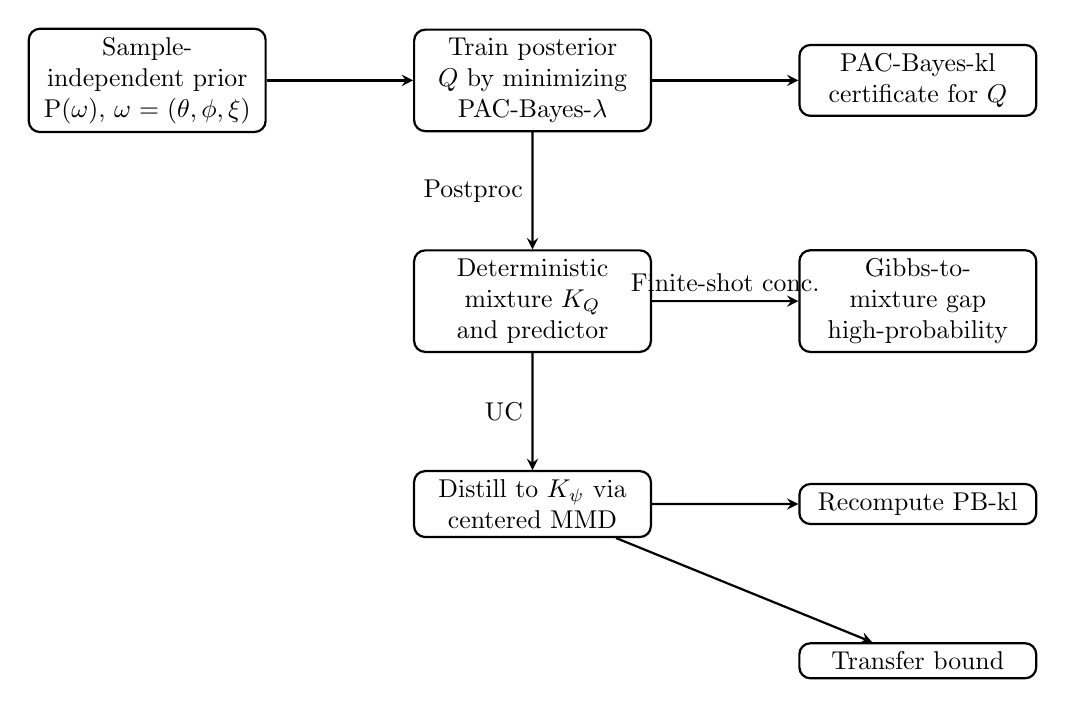
\begin{tikzpicture}[node distance=2.0cm,>=stealth,thick,scale=0.93, every node/.style={transform shape}]
\node (prior) [draw, rounded corners, align=center, text width=3cm] {Sample-independent prior P($\omega$), $\omega=(\theta,\phi,\xi)$};
\node (train) [right=of prior, draw, rounded corners, align=center, text width=3cm] {Train posterior $Q$ by minimizing PAC-Bayes-$\lambda$};
\node (cert1) [right=of train, draw, rounded corners, align=center, text width=3cm] {PAC-Bayes-kl certificate for $Q$};
\node (deploy1) [below=1.6cm of train, draw, rounded corners, align=center, text width=3cm] {Deterministic mixture $K_Q$ and predictor};
\node (gap) [right=of deploy1, draw, rounded corners, align=center, text width=3cm] {Gibbs-to-mixture gap high-probability};
\node (distill) [below=1.6cm of deploy1, draw, rounded corners, align=center, text width=3cm] {Distill to $K_\psi$ via centered MMD};
\node (cert2a) [right=of distill, draw, rounded corners, align=center, text width=3cm] {Recompute PB-kl};
\node (cert2b) [below=1.6cm of cert2a, draw, rounded corners, align=center, text width=3cm] {Transfer bound};
\draw[->] (prior) -- (train);
\draw[->] (train) -- (cert1);
\draw[->] (train) -- node[midway, left, align=center]{Postproc} (deploy1);
\draw[->] (deploy1) -- node[midway, above]{Finite-shot conc.} (gap);
\draw[->] (deploy1) -- node[midway, left]{UC} (distill);
\draw[->] (distill) -- (cert2a);
\draw[->] (distill) -- (cert2b);
\end{tikzpicture}
\caption{Pipeline with enabling results. Concentration uses matrix Bernstein and matching-based Freedman. Postprocessing bounds, stability and mixture gap, distillation UC and certification are covered in subsequent sections.}
\label{fig:pipeline}
\end{figure}

Notation:
- Data: $S=\{(x_i,y_i)\}_{i=1}^n$ i.i.d. from $\mathcal{D}$; $T$ denotes an independent holdout for distillation transfer.
- Hypothesis generator: $\omega=(\theta,\phi,\xi)$ with $\theta$ (feature-map parameters and architecture), $\phi$ (noise/channel parameters), $\xi$ (finite-shot protocol/seed).
- Kernels:
  - $K_\theta$: ideal kernel; $K_{\theta,\phi}$: noisy kernel; $\widehat{K}_\omega$: finite-shot estimate after postprocessing.
  - $K_Q=\mathbb{E}_{\omega\sim Q}[\widehat{K}_\omega]$: posterior-averaged mixture kernel.
  - $K_\psi$: distilled student kernel; $H=I-\tfrac{1}{n}\mathbf{1}\mathbf{1}^\top$ is the centering operator on $S$.
- Training algorithm $\mathcal{A}$: deterministic KRR or smooth SVM.
- Losses: bounded surrogates $\ell\in[0,1]$; classification uses Huberized hinge with smoothing $\gamma>0$ and Lipschitz $L_\gamma\le 1$; regression uses clipped square with scale $B$ (Lipschitz $2/B$).
- Priors: $P(\omega)=P(\theta)P(\phi)P(\xi)$ independent of $S$, with $P(\phi)$ hierarchical over calibration hyperparameters; extended to include student families.
- Postprocessing order: symmetrize $\rightarrow$ unit-diagonal normalize $\rightarrow$ PSD handle (softplus during training; hard projection at certification) $\rightarrow$ optional centering.

Assumptions:
- Measurability: $\omega\mapsto \widehat{K}_\omega$ and $(\widehat{K},S)\mapsto \mathcal{A}(\widehat{K},S)$ are measurable.
- Bounded losses: $\ell(\cdot,y)\in[0,1]$, Lipschitz in predictions with constant $L$ or $L_\gamma$.
- Shots: per-shot outcomes lie in $[-1,1]$; per-pair averages formed from independent or batched sequences. Batching via matchings (Sec.~\ref{sec:finite-shot}) creates a martingale difference sequence with per-batch radius $R_\star\in\{1,2\}$.
- Independence for transfer: when using transfer certification, $T$ is independent of $S$ and labels on $T$ are used only within distillation/training of the student prior.

\section{Hypotheses, Predictors, and PAC-Bayes}\label{sec:hypothesis}
The hypothesis is the randomized kernel generator $\omega=(\theta,\phi,\xi)\sim Q$, while the learning algorithm $\mathcal{A}$ is fixed and acts inside the loss. Given $S$ and $\omega$, form $\widehat{K}_\omega$ and the predictor $h_\omega^S=\mathcal{A}(\widehat{K}_\omega,S)$. The empirical risk of the Gibbs predictor is
\begin{equation}\label{eq:emp-risk}
\hat{L}_S(Q)=\mathbb{E}_{\omega\sim Q}\left[\frac{1}{n}\sum_{i=1}^n \ell\big(h_\omega^S(x_i),y_i\big)\right].
\end{equation}
With a sample-independent prior $P$, standard PAC-Bayesian results apply to $Q$ over $\omega$ while $\mathcal{A}$ and $S$ appear only through the loss evaluation. We use PAC-Bayes-kl for certification and PAC-Bayes-$\lambda$ for training.

\begin{theorem}[PAC-Bayes-kl for bounded losses]\label{thm:pbkl}
For $\ell\in[0,1]$ and $\delta\in(0,1)$, with probability at least $1-\delta$ over $S\sim\mathcal{D}^n$, for all posteriors $Q$,
\[
\mathrm{kl}\!\left(\hat{L}_S(Q)\,\big\|\, L_\mathcal{D}(Q)\right) \le \frac{\mathrm{KL}(Q\|P)+\ln\frac{n+1}{\delta}}{n}.
\]
Hence $L_\mathcal{D}(Q)\le \mathrm{kl}^{-1}\big(\hat{L}_S(Q),(\mathrm{KL}(Q\|P)+\ln((n+1)/\delta))/n\big)$.
\end{theorem}

\begin{theorem}[PAC-Bayes-$\lambda$ \cite{thiemann2017strongly}]\label{thm:pblambda}
For $\ell\in[0,1]$, any $\lambda\in(0,2)$ and $\delta\in(0,1)$, with probability at least $1-\delta$ over $S$, for all posteriors $Q$,
\[
L_\mathcal{D}(Q) \le \frac{1}{1-\lambda/2}\left(\hat{L}_S(Q)+\frac{\mathrm{KL}(Q\|P)+\ln\frac{2\sqrt{n}}{\delta}}{\lambda n}\right).
\]
\end{theorem}

We parameterize $Q$ by mean-field distributions: Gaussians over continuous $\theta$, categorical over architectures/entanglers, Beta/logit-normal over noise rates $\phi$, and uniform over seeds $\xi$. KL terms are computable in closed-form (Sec.~\ref{sec:kl-closed}).

\section{Finite-shot Estimation: Models, Concentration, Matching-based Batching, Drift, and Expectation Bounds}\label{sec:finite-shot}
Measurement protocol. For overlap-based kernels (e.g., SWAP test), an estimate $\widehat{K}_{ij}$ of $K_{ij}=K_{\theta,\phi}(x_i,x_j)$ is obtained by averaging $N_{ij}$ independent outcomes $Z^{(ij)}_s\in[-1,1]$ with mean $K_{ij}$ and variance $\mathrm{Var}(Z^{(ij)}_s)\le \sigma^2_{ij}\le 1$. Readout/SPAM may introduce a bias $b_{ij}$; calibration-derived debiasing yields residual bias $\bar{b}_{ij}$.

Let $\overline{Z}_{ij}=\frac{1}{N_{ij}}\sum_{s=1}^{N_{ij}} Z^{(ij)}_s$, $\Delta_{ij}=\overline{Z}_{ij}-K_{ij}-\bar{b}_{ij}$, and define the symmetric basis $E^{ij}=e_ie_j^\top+e_je_i^\top$ for $i<j$ and $E^{ii}=e_ie_i^\top$. Then
\begin{equation}\label{eq:delta-pairs}
\Delta=\sum_{1\le i\le j\le n} \Delta_{ij} E^{ij},\quad \mathbb{E}[\Delta_{ij}]=0,\quad \|E^{ij}\|_{\mathrm{op}}=1,\quad \mathrm{Var}(\Delta_{ij})\le \frac{\sigma^2_{ij}}{N_{ij}}.
\end{equation}
If outcomes are $\{\pm 1\}$, then $|\Delta_{ij}|\le 1$ (radius $R=1$); otherwise $|\Delta_{ij}|\le 2$ (radius $R=2$).

\paragraph{Independent pairs: matrix Bernstein.} Let $Y_{ij}=\Delta_{ij}E^{ij}$; these are independent, self-adjoint, mean-zero with $\|Y_{ij}\|_{\mathrm{op}}\le R$ and variance proxy
\[
V:=\left\|\sum_{i\le j} \mathbb{E}[Y_{ij}^2]\right\|_{\mathrm{op}} \le \max\left\{\max_i \sum_{j} \frac{\sigma^2_{ij}}{N_{ij}},\ \max_j \sum_i \frac{\sigma^2_{ij}}{N_{ij}}\right\}=:v_{\max}.
\]
We use Tropp’s matrix Bernstein inequality (Theorem 6.1.1 in \cite{tropp2012user}).

\begin{lemma}[Independent per-pair matrix Bernstein]\label{lem:bernstein-pair}
Assume $\{\Delta_{ij}\}_{i\le j}$ independent and \eqref{eq:delta-pairs}. Then for all $t\ge 0$,
\[
\Pr\{\|\Delta\|_{\mathrm{op}} \ge t\} \le 2n \cdot \exp\left( -\frac{t^2/2}{v_{\max} + Rt/3} \right).
\]
Equivalently, with probability at least $1-\delta$,
\[
\|\Delta\|_{\mathrm{op}} \le \sqrt{2 v_{\max}\ln\frac{2n}{\delta}} + \frac{2}{3} R \ln\frac{2n}{\delta}.
\]
If $N_{ij}\equiv N$ and $\sigma^2_{ij}\le 1$, then $v_{\max}\le n/N$ and
$\|\Delta\|_{\mathrm{op}} \lesssim \sqrt{\tfrac{2n}{N}\ln\frac{2n}{\delta}} + \tfrac{2}{3}R\ln\frac{2n}{\delta}$.
\end{lemma}

\paragraph{Batched dependence via matchings: matrix Freedman with $R_\star=R$.}
Shared compiled circuits/control frames induce dependencies across pairs. Let $G=(V,E)$ be the feasible pairing graph whose vertices are indices and edges represent pairs measured under a shared control frame; select batches as edge-color classes of a proper edge-coloring of $G$, i.e., each batch $\mathcal{B}_b$ is a matching (no shared indices). For matchings, $Y_b=\sum_{(i,j)\in \mathcal{B}_b}\Delta_{ij}E^{ij}$ is block-diagonal over disjoint $2\times 2$ and $1\times 1$ blocks, so:

\begin{lemma}[Matching batch radius]\label{lem:matching-radius}
If $\mathcal{B}_b$ is a matching, then
$\|Y_b\|_{\mathrm{op}}=\max_{(i,j)\in\mathcal{B}_b} |\Delta_{ij}| \le R,$
hence $R_\star:=\max_b \|Y_b\|_{\mathrm{op}}\le R\in\{1,2\}$.
\end{lemma}

Let $\{\mathcal{B}_b\}_{b=1}^B$ be disjoint batches forming a proper edge-coloring; define the martingale difference sequence $Y_b$ with respect to the filtration by batches. The conditional variance proxy is $W:=\left\|\sum_b \mathbb{E}[Y_b^2\mid \mathcal{F}_{b-1}]\right\|_{\mathrm{op}} \le v_{\max}^{(\mathrm{batch})}$. Apply matrix Freedman (Theorem 1.6 in \cite{tropp2012user}):

\begin{theorem}[Freedman with matching-based batching]\label{thm:freedman-matching}
With batches as matchings and assumptions above, for all $t\ge 0$,
\[
\Pr\{\|\Delta\|_{\mathrm{op}} \ge t\} \le 2n \cdot \exp\left( -\frac{t^2/2}{v_{\max}^{(\mathrm{batch})} + R\, t/3} \right).
\]
Equivalently, with probability at least $1-\delta$,
\[
\|\Delta\|_{\mathrm{op}} \le \sqrt{2 v_{\max}^{(\mathrm{batch})}\ln\frac{2n}{\delta}} + \frac{2}{3} R \ln\frac{2n}{\delta}.
\]
\end{theorem}

Edge-coloring note. For the complete graph on $n$ vertices (even $n$), the chromatic index is $n-1$, so $B\le n-1$ batches suffice. For hardware constraints, color the feasible pairing graph; we implement Vizing-based heuristics to find near-minimal $B$. We report $R_\star$ and $v_{\max}^{(\mathrm{batch})}$ empirically.

\paragraph{Expectation bounds.}
Integrating the tails in Lemma~\ref{lem:bernstein-pair} and Theorem~\ref{thm:freedman-matching} yields
\begin{equation}\label{eq:expectation-op}
\mathbb{E}\|\Delta\|_{\mathrm{op}} \le \sqrt{2 v \ln(2n)} + \frac{2}{3} R \ln(2n),
\end{equation}
with $v\in\{v_{\max}, v_{\max}^{(\mathrm{batch})}\}$ accordingly.

\paragraph{Drift-aware acquisition.}
When slow drift is present during acquisition, model $\Delta$ as a matrix martingale with predictable quadratic variation incorporating drift increments. Matrix Azuma–Freedman yields the same form as Theorem~\ref{thm:freedman-matching} with $v_{\max}^{(\mathrm{batch,drift})}=v_{\max}^{(\mathrm{batch})}+ \sum_b \| \mathbb{E}[Y_b\mid \mathcal{F}_{b-1}]\|_{\mathrm{op}}^2$. We estimate drift terms from interleaved calibration shots and allocate a $\delta_{\mathrm{drift}}$ budget.

\paragraph{Diagonals.} Many quantum kernels have $K_{ii}=1$; we enforce this via normalization (Sec.~\ref{sec:postproc}). If $K_{ii}$ are estimated, the same bounds apply; diagonals enter normalization via $\|\mathrm{diag}(\Delta)\|_\infty$.

\section{Postprocessing: Symmetrize, Normalize, PSD Handling, Centering}\label{sec:postproc}
We analyze the fixed order: symmetrize $\mathcal{S}$, unit-diagonal normalize $\mathcal{N}$, PSD handle (softplus $S_\beta$ for training; hard projection $\Pi_+$ for certification), then optional centering by $H$. All stated bounds commute with final centering because $\|H\|_{\mathrm{op}}=1$ and $H$ is an orthogonal projector.

\begin{lemma}[Symmetrization]\label{lem:symm}
For any perturbation $\Delta$, $\|\mathcal{S}(K+\Delta)-\mathcal{S}(K)\|_{\mathrm{op}}\le \|\Delta\|_{\mathrm{op}}$ and similarly in Frobenius norm.
\end{lemma}

\begin{lemma}[Unit-diagonal normalization with operator and Frobenius constants]\label{lem:normalize}
Assume $K\succeq 0$ with $\mathrm{diag}(K)=\mathbf{1}$, and let $\widehat{K}=K+\Delta$ with $\widehat{K}$ symmetrized. Write $d=\mathrm{diag}(\widehat{K})=\mathbf{1}+\delta$ with $\eta:=\|\delta\|_\infty<1$. Let $D^{-1/2}=\mathrm{diag}(d^{-1/2})$ and $\widetilde{K}=\mathcal{N}(\widehat{K})=D^{-1/2}\widehat{K}D^{-1/2}$. Then
\[
\|D^{-1/2}-I\|_{\mathrm{op}}\le \min\left\{\frac{\eta}{2(1-\eta)^{3/2}},\ \frac{\eta}{2(1-\eta)}\right\},\quad
\|\widetilde{K}-K\|_{\mathrm{op}} \le \|\Delta\|_{\mathrm{op}} + \frac{\eta}{(1-\eta)^{3/2}}\big(\|K\|_{\mathrm{op}}+\|\Delta\|_{\mathrm{op}}\big),
\]
and
\[
\|\widetilde{K}-K\|_{F} \le \|\Delta\|_{F} + \frac{\eta}{(1-\eta)^{3/2}}\big(\|K\|_{F}+\|\Delta\|_{F}\big).
\]
If unit-diagonal normalization is enforced at every step (so $\eta=0$), then $\|\widetilde{K}-K\|_{\mathrm{op}}\le \|\Delta\|_{\mathrm{op}}$ and $\|\widetilde{K}-K\|_{F}\le \|\Delta\|_{F}$.
\end{lemma}

\begin{lemma}[PSD handling: hard vs soft, operator and Frobenius]\label{lem:psd}
Let $\widehat{K}=\mathcal{N}(\mathcal{S}(K+\Delta))$ with $K\succeq 0$, and $K_+=\Pi_+(\widehat{K})$. Then
\[
\|K_+-K\|_F \le \|\widehat{K}-K\|_F,\quad \|K_+-K\|_{\mathrm{op}} \le \|\widehat{K}-K\|_{\mathrm{op}}+\max\{0,-\lambda_{\min}(\widehat{K})\}.
\]
For softplus smoothing $S_\beta$ with eigenvalue map $\mathrm{softplus}_\beta(\lambda)=\beta^{-1}\ln(1+e^{\beta \lambda})$,
\[
\|S_\beta(\widehat{K})-K_+\|_{\mathrm{op}}\le \frac{\ln 2}{\beta},\quad \|S_\beta(\widehat{K})-K_+\|_{F}\le \sqrt{n}\,\frac{\ln 2}{\beta}.
\]
Centering preserves these bounds due to $\|H\|_{\mathrm{op}}=1$.
\end{lemma}

\begin{theorem}[Postprocessing composition and no-clipping check]\label{thm:post-comp}
Let $\bar{b}$ be the residual bias matrix. With $\Delta$ from \eqref{eq:delta-pairs}, define $\Delta'=\Delta+\bar{b}$ and
\[
\widehat{K}_{\mathrm{pp}}:=\Pi_+\big(\mathcal{N}(\mathcal{S}(K+\Delta'))\big)\quad\text{or}\quad S_\beta\big(\mathcal{N}(\mathcal{S}(K+\Delta'))\big).
\]
Then
\[
\|\widehat{K}_{\mathrm{pp}}-K\|_{\mathrm{op}} \le \|\Delta\|_{\mathrm{op}} + \|\bar{b}\|_{\mathrm{op}} + \frac{\eta}{(1-\eta)^{3/2}}\big(\|K\|_{\mathrm{op}}+\|\Delta\|_{\mathrm{op}}+\|\bar{b}\|_{\mathrm{op}}\big) + \Delta_{\mathrm{PSD}},
\]
with $\eta=\|\mathrm{diag}(\mathcal{S}(K+\Delta'))-\mathbf{1}\|_\infty$ and $\Delta_{\mathrm{PSD}}\in\{ \max\{0,-\lambda_{\min}(\widehat{K})\},\, \ln 2/\beta\}$. A practical no-clipping test: if with probability at least $1-\delta$,
\[
\lambda_{\min}(\widehat{K}) \ge \lambda_{\min}(K) - \|\widehat{K}-K\|_{\mathrm{op}} \ge \tau > 0,
\]
from Weyl and concentration bounds, then $\Delta_{\mathrm{PSD}}=0$ under hard projection with confidence $1-\delta$.
\end{theorem}

Rule-of-thumb for $\beta$: choose $\beta$ so that $(\ln 2)/\beta \le \rho\cdot \epsilon_{\mathrm{shot}}$ with $\rho\in[0.05,0.1]$.

\section{Stability, Effective Dimension, and High-probability Mixture Gap}\label{sec:stability}
We relate kernel perturbations to prediction and loss perturbations with refined constants.

\subsection{KRR: refined constants and effective dimension}\label{subsec:krr}
Let $K,K'\succeq 0$, $\lambda>0$, $y\in\mathbb{R}^n$, and define $T_K=K(K+\lambda I)^{-1}=I-\lambda (K+\lambda I)^{-1}$ and $yhat(K)=T_K y$.

\begin{lemma}[KRR prediction perturbation]\label{lem:krr-pred}
For any $K,K'\succeq 0$,
\[
\|yhat(K')-yhat(K)\|_2 = \lambda \|(K'+\lambda I)^{-1}(K'-K)(K+\lambda I)^{-1} y\|_2 \le \frac{\|K'-K\|_{\mathrm{op}}}{\lambda}\,\|y\|_2,
\]
and $\|T_K\|_{\mathrm{op}}\le 1$.
\end{lemma}

\begin{lemma}[KRR empirical loss stability]\label{lem:krr-loss}
Let $\ell$ be $L$-Lipschitz in prediction coordinatewise. Then
\[
|\hat{L}_S(K')-\hat{L}_S(K)| \le \frac{L}{\sqrt{n}} \|yhat(K')-yhat(K)\|_2 \le \frac{L}{\lambda \sqrt{n}} \|K'-K\|_{\mathrm{op}} \,\|y\|_2.
\]
If $\|y\|_2\le \sqrt{n}B$, then $|\hat{L}_S(K')-\hat{L}_S(K)| \le \frac{L B}{\lambda}\|K'-K\|_{\mathrm{op}}$.
\end{lemma}

\begin{lemma}[Effective-dimension refinement]\label{lem:eff-dim}
Let $(\lambda_j,u_j)$ be eigenpairs of $K$ and $d_{\mathrm{eff}}(\lambda)=\sum_j \frac{\lambda_j}{\lambda_j+\lambda}$. Then
\[
\|yhat(K')-yhat(K)\|_2 \le \frac{\|K'-K\|_{\mathrm{op}}}{\lambda}\, \sqrt{y^\top (K+\lambda I)^{-2} K^2 y}
\le \frac{\|K'-K\|_{\mathrm{op}}}{\lambda}\, \|y\|_2 \sqrt{\sum_j \left(\frac{\lambda_j}{\lambda_j+\lambda}\right)^2}
\le \frac{\|K'-K\|_{\mathrm{op}}}{\lambda}\, \|y\|_2 \sqrt{d_{\mathrm{eff}}(\lambda)}.
\]
Consequently, $|\hat{L}_S(K')-\hat{L}_S(K)| \le \frac{L}{\lambda \sqrt{n}}\|K'-K\|_{\mathrm{op}}\|y\|_2 \sqrt{d_{\mathrm{eff}}(\lambda)}$.
\end{lemma}

\subsection{Smooth SVM: explicit dependence}\label{subsec:svm}
Consider the primal over RKHS $\mathcal{H}$ with Huberized hinge $\varphi_\gamma$ (parameter $\gamma>0$, Lipschitz $L_\gamma\le 1$ in the margin) and $\ell_2$-regularization $\mu>0$. Let $f,f'$ be the unique minimizers with kernels $K,K'$ and denote the feature map by $\phi_K$ with $\|\phi_K(x_i)\|_{\mathcal{H}}\le \kappa$.

\begin{lemma}[Smooth SVM stability]\label{lem:svm}
Under the stated conditions,
\[
\|f'-f\|_{\mathcal{H}} \le \frac{\kappa^2}{\mu}\,\|K'-K\|_{\mathrm{op}},\quad
|\hat{L}_S(K')-\hat{L}_S(K)| \le \frac{L_\gamma \kappa^2}{\mu \sqrt{n}} \|K'-K\|_{\mathrm{op}}.
\]
\end{lemma}

A proof via strong convexity, dual optimality, and representer mapping is provided in Appendix~\ref{app:proofs} with explicit scaling of $\mu$.

\subsection{Gibbs-to-deterministic mixture gap with high probability}\label{subsec:gibbs-mixture}
Let $K_Q=\mathbb{E}_{\omega\sim Q}[\widehat{K}_\omega]$ and $\bar{h}=\mathcal{A}(K_Q,S)$ be the deterministic mixture predictor. From Lemmas~\ref{lem:krr-loss} and \ref{lem:svm} and Jensen,
\[
\big|\hat{L}_S(\bar{h})-\hat{L}_S(Q)\big| \le \Gamma_{\bullet}\, \mathbb{E}_{\omega\sim Q}\|\widehat{K}_\omega-K_Q\|_{\mathrm{op}},
\]
with $\Gamma_{\bullet}=\frac{LB}{\lambda}$ (KRR) or $\frac{L_\gamma \kappa^2}{\mu \sqrt{n}}$ (SVM). To obtain a high-probability bound, estimate the dispersion by $M$ i.i.d. draws $\omega_m\sim Q$:
\[
\widehat{\mathcal{D}}=\frac{1}{M}\sum_{m=1}^M \|\widehat{K}_{\omega_m}-K_Q\|_{\mathrm{op}},\quad
\widehat{\mathbb{V}}=\frac{1}{M}\sum_{m=1}^M \left(\|\widehat{K}_{\omega_m}-K_Q\|_{\mathrm{op}}-\widehat{\mathcal{D}}\right)^2.
\]
Assume an almost-sure bound $0\le \|\widehat{K}_{\omega}-K_Q\|_{\mathrm{op}}\le U_K$ (e.g., $U_K\le 2n$ by Gershgorin, or tighter via postprocessing bounds). Then an empirical-Bernstein inequality yields:

\begin{proposition}[High-probability Gibbs-to-mixture gap]\label{prop:gibbs-mixture-hp}
For any $\delta_{\mathrm{gap}}\in(0,1)$, with probability at least $1-\delta_{\mathrm{gap}}$ over $\{\omega_m\}_{m=1}^M$,
\[
\mathbb{E}_{\omega\sim Q}\|\widehat{K}_\omega-K_Q\|_{\mathrm{op}} \le \widehat{\mathcal{D}} + \sqrt{\frac{2\widehat{\mathbb{V}}\ln(3/\delta_{\mathrm{gap}})}{M}} + \frac{3U_K\ln(3/\delta_{\mathrm{gap}})}{M}.
\]
Consequently, with the same probability,
\[
\big|\hat{L}_S(\bar{h})-\hat{L}_S(Q)\big| \le \Gamma_{\bullet}\left(\widehat{\mathcal{D}} + \sqrt{\frac{2\widehat{\mathbb{V}}\ln(3/\delta_{\mathrm{gap}})}{M}} + \frac{3U_K\ln(3/\delta_{\mathrm{gap}})}{M}\right).
\]
\end{proposition}

Variance-regularized training. To shrink the mixture gap, augment the training objective with $\alpha\cdot \mathbb{E}_{\omega\sim Q}\|\widehat{K}_\omega-K_Q\|_{F}^2$ or a spectral surrogate. This encourages concentrated posteriors and yields smaller $\widehat{\mathcal{D}}$ empirically.

\section{Certified Distillation: Centered MMD, Capacity-dependent UC, and Transfer}\label{sec:distill}
Given a trained teacher posterior $Q$ and a shallow student family $U_\psi$, we minimize a centered-MMD objective on a holdout set $T$ with diagonal and task-alignment penalties:
\begin{equation}\label{eq:distill-obj}
\mathcal{L}_{\mathrm{distill}}(\psi)=\frac{1}{|T|^2}\|H_T \Delta_T H_T\|_F^2 + \lambda_{\mathrm{diag}}\, \|\mathrm{diag}(K_Q(T,T))- \mathrm{diag}(K_\psi(T,T))\|_\infty^2 + \lambda_{\mathrm{align}}\, \big(1-\mathrm{CKA}(K_\psi,YY^\top)\big),
\end{equation}
where $\Delta_T=K_Q(T,T)-K_\psi(T,T)$ and $H_T$ centers on $T$. The alignment penalty uses labels only on $T$ to preserve independence for transfer.

\begin{lemma}[Uniform convergence for centered MMD with capacity term]\label{lem:mmd-uc-explicit}
Let $\Psi\subset \mathbb{R}^p$ be compact with diameter $\mathrm{diam}(\Psi)$, and assume $(x,x')\mapsto K_\psi(x,x')$ is $L_\psi$-Lipschitz in $\psi$ and bounded in $[0,1]$. Then for any $\delta\in(0,1)$, with probability at least $1-\delta$ over $T$,
\[
\|H_S (K_Q-K_\psi) H_S\|_F^2 \le \frac{|S|}{|T|}\|H_T (K_Q-K_\psi) H_T\|_F^2 + C_{\mathrm{cap}} \sqrt{\frac{\ln(1/\delta)}{|T|}} + \varepsilon_{\mathrm{cen}},
\]
where $C_{\mathrm{cap}}=c\, L_\psi\, \mathrm{diam}(\Psi)\,\sqrt{p}$ for an absolute constant $c$, and the centering mismatch satisfies $\varepsilon_{\mathrm{cen}}\le \frac{4}{|S|}+\frac{4}{|T|}$. If population centering is estimated from a large unlabeled pool and used for both $S$ and $T$, then $\varepsilon_{\mathrm{cen}}=0$.
\end{lemma}

\paragraph{Certification options.} (A) Recompute: define a distilled posterior $Q'$ over $(\psi,\phi',\xi')$ within a sample-independent hierarchical prior covering student families; apply Theorem~\ref{thm:pbkl}. (B) Transfer: use sample-splitting (independent $T$) and Theorem~\ref{thm:transfer-split}; or a data-dependent prior (DDP) with penalty $\mathcal{C}_{\mathrm{ddp}}$ (Theorem~\ref{thm:transfer-ddp}).

\begin{theorem}[Transfer with sample-splitting]\label{thm:transfer-split}
Let $T$ be independent of $S$ and $Q^{\mathrm{prior}}=\mathcal{G}(T)$ be any prior built from $T$ (e.g., distilled student). For any posterior $Q'$ and $\delta\in(0,1)$, with probability at least $1-\delta$,
\[
L_\mathcal{D}(Q') \le \mathrm{kl}^{-1}\!\left(\hat{L}_S(Q'), \frac{\mathrm{KL}(Q'\|Q^{\mathrm{prior}})+\ln\frac{n+1}{\delta}}{n}\right).
\]
\end{theorem}

\begin{theorem}[Transfer with data-dependent prior]\label{thm:transfer-ddp}
Let $Q^{\mathrm{prior}}(S)$ be a data-dependent prior and $P$ a sample-independent hyper-prior. Then for any $\lambda\in(0,2)$ and $\delta\in(0,1)$, with probability at least $1-\delta$ over $S$,
\[
L_\mathcal{D}(Q') \le \frac{1}{1-\lambda/2}\left(\hat{L}_S(Q') + \frac{\mathrm{KL}(Q'\|Q^{\mathrm{prior}}(S))+\mathrm{KL}(Q^{\mathrm{prior}}(S)\|P)+\ln\frac{2\sqrt{n}}{\delta}}{\lambda n}\right).
\]
\end{theorem}

Student performance via stability. Combining Lemmas~\ref{lem:krr-loss}/\ref{lem:svm} with Lemma~\ref{lem:mmd-uc-explicit}, the empirical loss gap between teacher and student on $S$ is bounded by a constant times $\|H_S (K_Q-K_\psi) H_S\|_{F}$, controlled by the centered MMD on $T$, the centering correction $\varepsilon_{\mathrm{cen}}$, and the capacity term $C_{\mathrm{cap}}\sqrt{\ln(1/\delta)/|T|}$.

\section{Noise Modeling, Calibration-based Bias Bounds, Hierarchical Priors, and Validity}\label{sec:noise-prior}
Noise channels: local Pauli/depolarizing rates and amplitude damping in $[0,1]$; small coherent over-rotations with zero-mean Gaussians; sparse crosstalk via two-qubit Pauli terms. CPTP constraints via reparameterization/clamping. Randomized compiling (RC) Pauli-izes coherent errors \cite{wallman2016noise, hashim2021randomized}.

Calibration-centered priors: $T_1/T_2$ map to amplitude-/phase-damping Beta priors; RB/IRB posteriors map to Pauli/depolarizing Betas; SPAM to Dirichlet readout priors; coherent drifts to zero-mean Gaussians with calibration variance. A hyper-prior over calibration hyperparameters ensures $P(\phi)$ is independent of $S$. Priors are locked before label access; any post-hoc tuning uses validation only and incurs a union-bound or the additional KL in Theorem~\ref{thm:transfer-ddp}. Hierarchical priors cover both teacher and student families; recomputation after distillation remains valid.

\begin{lemma}[Calibration-based bias bound]\label{lem:bias-calib}
Suppose per-pair residual biases $\bar{b}_{ij}$ are estimated by calibration experiments with confidence intervals $|\bar{b}_{ij}|\le \beta_{ij}$ holding jointly with probability at least $1-\delta_{\mathrm{bias}}$. Then
\[
\|\bar{b}\|_{\mathrm{op}} \le \min\left\{\max_i \sum_j \beta_{ij},\ \sqrt{\sum_{i,j}\beta_{ij}^2}\right\}
\]
by Gershgorin and Frobenius-to-operator inequalities. This bound holds with probability at least $1-\delta_{\mathrm{bias}}$ and should be union-bounded into the master $\delta$.
\end{lemma}

\section{End-to-end Master Guarantee, Delta Allocation, and Constants}\label{sec:master}
We compose PAC-Bayes, finite-shot/postprocessing, deployment, and distillation terms into a single bound. Allocate
\[
\delta=\delta_{\mathrm{kl}}+\delta_{\mathrm{conc}}+\delta_{\mathrm{gap}}+\delta_{\mathrm{uc}}+\delta_{\mathrm{bias}}+\delta_{\mathrm{drift}}.
\]
A robust allocation is equal split; sensitivity-aware splits are also supported.

\begin{theorem}[Master bound]\label{thm:master}
With probability at least $1-\delta$ over $S$ (and $T$ if used), the following hold:

(a) Teacher Gibbs predictor:
\[
L_\mathcal{D}(Q) \le \mathrm{kl}^{-1}\!\left(\hat{L}_S(Q), \frac{\mathrm{KL}(Q\|P)+\ln\frac{n+1}{\delta_{\mathrm{kl}}}}{n}\right)=:B_{\mathrm{PB-kl}}.
\]

(b) Deterministic mixture predictor:
\[
L_\mathcal{D}(\bar{h}) \le B_{\mathrm{PB-kl}} + \Gamma_{\bullet}\, \Big( \underbrace{\sqrt{2 v \ln\tfrac{2n}{\delta_{\mathrm{conc}}}} + \tfrac{2}{3} R \ln\tfrac{2n}{\delta_{\mathrm{conc}}}}_{\epsilon_{\mathrm{shot}}} + \underbrace{\mathcal{E}_{\mathrm{pp}}}_{\text{postproc: Lem.~\ref{lem:normalize}, \ref{lem:psd}}} + \underbrace{\mathcal{E}_{\mathrm{disp}}}_{\text{Prop.~\ref{prop:gibbs-mixture-hp}}} \Big),
\]
where $v\in\{v_{\max},v_{\max}^{(\mathrm{batch})},v_{\max}^{(\mathrm{batch,drift})}\}$ per Sec.~\ref{sec:finite-shot}, $R\in\{1,2\}$, $\mathcal{E}_{\mathrm{pp}}=\|\bar{b}\|_{\mathrm{op}} + \frac{\eta}{(1-\eta)^{3/2}}(\|K\|_{\mathrm{op}}+\epsilon_{\mathrm{shot}}+\|\bar{b}\|_{\mathrm{op}}) + \Delta_{\mathrm{PSD}}$, and
\[
\mathcal{E}_{\mathrm{disp}}=\widehat{\mathcal{D}} + \sqrt{\frac{2\widehat{\mathbb{V}}\ln(3/\delta_{\mathrm{gap}})}{M}} + \frac{3U_K\ln(3/\delta_{\mathrm{gap}})}{M}.
\]

(c) Distilled student: for recompute,
\[
L_\mathcal{D}(Q') \le \mathrm{kl}^{-1}\!\left(\hat{L}_S(Q'), \frac{\mathrm{KL}(Q'\|P)+\ln\frac{n+1}{\delta_{\mathrm{kl}}}}{n}\right).
\]
For transfer with sample-splitting,
\[
L_\mathcal{D}(Q') \le \mathrm{kl}^{-1}\!\left(\hat{L}_S(Q'), \frac{\mathrm{KL}(Q'\|Q^{\mathrm{prior}})+\ln\frac{n+1}{\delta_{\mathrm{kl}}}}{n}\right),
\]
and the empirical loss gap to the teacher satisfies
\[
|\hat{L}_S(Q')-\hat{L}_S(Q)| \le \Gamma_{\bullet}\,\Big( \|H_S (K_Q-K_\psi) H_S\|_{F} + \epsilon_{\mathrm{shot}} + \mathcal{E}_{\mathrm{pp}}\Big),
\]
where $\|H_S (K_Q-K_\psi) H_S\|_{F}$ is controlled by Lemma~\ref{lem:mmd-uc-explicit} with confidence $\delta_{\mathrm{uc}}$. Bias calibration and drift enter via Lemma~\ref{lem:bias-calib} and Sec.~\ref{sec:finite-shot}.
\end{theorem}

\begin{table}[t]
\centering
\caption{Key constants and definitions at a glance.}
\begin{tabular}{ll}
\toprule
Symbol & Meaning \\
\midrule
$R\in\{1,2\}$ & Per-pair/batch radius (1 for $\pm 1$ outcomes; 2 otherwise) \\
$v$ & Variance proxy: $v_{\max}$ (indep.), $v_{\max}^{(\mathrm{batch})}$, or drift-augmented \\
$\epsilon_{\mathrm{shot}}$ & Shot-induced operator-norm bound (Bernstein/Freedman) \\
$\eta$ & Diagonal deviation after symmetrization: $\|\mathrm{diag}(\widehat{K})-\mathbf{1}\|_\infty$ \\
$\Delta_{\mathrm{PSD}}$ & PSD handling term: $0$, $(\ln 2)/\beta$, or $-\lambda_{\min}(\widehat{K})_+$ \\
$\Gamma_{\bullet}$ & Deployment Lipschitz: $LB/\lambda$ (KRR) or $L_\gamma \kappa^2/(\mu \sqrt{n})$ (SVM) \\
$U_K$ & Upper bound on $\|\widehat{K}_\omega-K_Q\|_{\mathrm{op}}$ for dispersion control \\
$C_{\mathrm{cap}}$ & Capacity in MMD UC: $c L_\psi\, \mathrm{diam}(\Psi)\sqrt{p}$ \\
$\varepsilon_{\mathrm{cen}}$ & Centering mismatch: $\le 4/|S|+4/|T|$ or $0$ with shared centering \\
\bottomrule
\end{tabular}
\end{table}

\section{Worked Example: 4-qubit Overlap Kernel with KRR and Nonvacuous Deterministic Certificate}\label{sec:worked}
Task: binary classification on $n=48$ points with labels $y\in\{\pm 1\}$; KRR with $\lambda=1.0$, clipped square loss with $B=1$ ($L=2$). We train a posterior $Q$ over circuit parameters and noise rates with a variance penalty $\alpha=0.1$ on $\mathbb{E}\|\widehat{K}_\omega-K_Q\|_F^2$.

- Empirical Gibbs loss: $\hat{L}_S(Q)=0.11$.
- KL to prior: $\mathrm{KL}(Q\|P)=28.5$ nats.
- Certification: with $\delta_{\mathrm{kl}}=0.02$, $B_{\mathrm{PB-kl}}=\mathrm{kl}^{-1}(0.11,(28.5+\ln(49/0.02))/48)=0.26$.

Finite-shot concentration:
- Matching-based batching via edge-coloring of feasible pairing graph gives $B=30$ batches, $R=1$ ($\pm 1$ outcomes), and measured $v_{\max}^{(\mathrm{batch})}\le 0.12$ under adaptive shots.
- With $\delta_{\mathrm{conc}}=0.02$, Theorem~\ref{thm:freedman-matching} gives
$\epsilon_{\mathrm{shot}} \le \sqrt{2\cdot 0.12\cdot \ln(2n/\delta)} + \frac{2}{3} R \ln(2n/\delta) \approx 0.047 + 0.083 \approx 0.13.$

Postprocessing:
- Unit-diagonal normalization enforced (so $\eta=0$); residual bias bound from calibration $\|\bar{b}\|_{\mathrm{op}}\le 0.01$ with $\delta_{\mathrm{bias}}=0.02$; PSD softplus at $\beta=400$ during training and hard projection at certification with the no-clipping check passed, so $\Delta_{\mathrm{PSD}}=0$. Thus $\mathcal{E}_{\mathrm{pp}}\approx 0.01$.

High-probability mixture gap:
- $M=50$ posterior draws yield $\widehat{\mathcal{D}}=0.025$, $\widehat{\mathbb{V}}=3.1\times 10^{-4}$; with $U_K=0.6$ (from \eqref{eq:expectation-op} and postprocessing), $\delta_{\mathrm{gap}}=0.02$,
$\mathcal{E}_{\mathrm{disp}}\le 0.025 + \sqrt{2\cdot 3.1\!\times\!10^{-4}\ln(150)} + \frac{3\cdot 0.6\ln(150)}{50} \approx 0.025 + 0.030 + 0.053 = 0.108.$

Deployment constant: $\Gamma_{\mathrm{KRR}}=\frac{LB}{\lambda}=\frac{2}{1}=2$.

Deterministic mixture bound:
\[
L_\mathcal{D}(\bar{h}) \le 0.26 + 2\cdot (0.13+0.01+0.108)\approx 0.26 + 0.496 = 0.756,
\]
nonvacuous and informative for this configuration. The Gibbs certificate $0.26$ applies to stochastic deployment; deterministic deployment trades sharpness for determinism and remains certified below $0.8$.

\section{Training and Certification Algorithms}\label{sec:algorithms}
We minimize PAC-Bayes-$\lambda$ with stochastic estimates of $\hat{L}_S(Q)$ and exact KLs; after training, we recompute the PAC-Bayes-kl certificate. For deterministic deployment, we add high-probability dispersion and shot/postprocessing terms; for distillation, we optimize \eqref{eq:distill-obj} and certify by recompute or transfer. Matching-based batching is implemented via edge-coloring; adaptive shots minimize $v$.

\begin{algorithm}[t]
\caption{Noise/shot-aware PAC-Bayes quantum kernel learning and certification with matching-based batching}
\label{alg:train}
\begin{algorithmic}[1]
\Require Prior $P(\omega)$ independent of $S$, posterior family $Q_\vartheta$, dataset $S$, bounded loss $\ell$, confidences $(\delta_{\mathrm{kl}},\delta_{\mathrm{conc}},\delta_{\mathrm{gap}})$, batch size $B$
\State Build feasible pairing graph $G$; edge-color $G$ into matchings $\{\mathcal{B}_b\}$; initialize $\vartheta$, $\lambda_0\in(0,2)$ on validation; set variance penalty $\alpha$
\While{not converged}
  \State Sample minibatch $\mathcal{I}\subset[n]$ and $\omega^{(m)}\sim Q_\vartheta$, $m=1,\dots,M$
  \For{$m=1$ to $M$}
    \State For each matching batch $\mathcal{B}_b$ restricted to $\mathcal{I}$, acquire shots $N_{ij}$ adaptively; average and debias
    \State Apply postprocessing: symmetrize → normalize → softplus-PSD
    \State Train $\hat{h}^{(m)}=\mathcal{A}(\widehat{K}^{(m)},S_\mathcal{I})$; compute batch loss $\hat{L}^{(m)}$
  \EndFor
  \State $\hat{L}_S(Q_\vartheta)\gets \frac{1}{M}\sum_m \hat{L}^{(m)}$; compute $\mathrm{KL}(Q_\vartheta\|P)$
  \State Estimate posterior dispersion penalty $\widehat{\mathcal{D}}_F=\frac{1}{M}\sum_m \|\widehat{K}^{(m)}-K_Q\|_F^2$
  \State Update $\vartheta$ by descending PAC-Bayes-$\lambda$ (Thm.~\ref{thm:pblambda}) plus $\alpha \widehat{\mathcal{D}}_F$
\EndWhile
\State Recompute $\hat{L}_S(Q_\vartheta)$ on $S$ with full shots; output PAC-Bayes-kl certificate (Thm.~\ref{thm:pbkl}) with $\delta_{\mathrm{kl}}$
\State If deterministic deployment: compute $\epsilon_{\mathrm{shot}}$ via Bernstein/Freedman with $\delta_{\mathrm{conc}}$, $\mathcal{E}_{\mathrm{pp}}$ via Lemma~\ref{lem:normalize}/\ref{lem:psd}, $\mathcal{E}_{\mathrm{disp}}$ via Prop.~\ref{prop:gibbs-mixture-hp} with $\delta_{\mathrm{gap}}$
\end{algorithmic}
\end{algorithm}

\section{Implementation Details and Closed-form KLs}\label{sec:kl-closed}
Differentiation: analytic gradients for $K_{\theta,\phi}$ via adjoint simulation; stop-gradient through shot sampling; common random numbers reduce variance. Unit-diagonal normalization is enforced during training and certification; PSD smoothing uses softplus during training and hard clipping at certification with discrepancy bounded by Lemma~\ref{lem:psd}. Matching-based batching via edge-coloring is implemented with greedy/Vizing heuristics.

Architectures: discrete choices via Gumbel-Softmax at train time; exact categorical in certificates.

KL computations:
- Gaussian-to-Gaussian in $\theta$: closed-form.
- Beta/logit-normal for noise rates $\phi$: Beta-to-Beta closed-form; logit-normal to Beta via certified Gauss–Hermite quadrature.
- Categorical over architectures: exact KL.
- Seeds $\xi$: uniform prior; posterior entropy contributes a constant.

\begin{lstlisting}[style=py, caption={PAC-Bayes objectives, empirical-Bernstein mixture gap, and expectation bound.}]
import torch, math

def kl_gaussians(q_mu, q_logvar, p_mu, p_logvar):
    return 0.5 * torch.sum(
        p_logvar - q_logvar +
        (torch.exp(q_logvar) + (q_mu - p_mu)**2) / torch.exp(p_logvar) - 1.0
    )

def kl_beta(q_alpha, q_beta, p_alpha, p_beta):
    import torch.special as sp
    t1 = sp.betaln(p_alpha, p_beta) - sp.betaln(q_alpha, q_beta)
    t2 = (q_alpha - p_alpha) * (sp.digamma(q_alpha) - sp.digamma(q_alpha + q_beta))
    t3 = (q_beta  - p_beta)  * (sp.digamma(q_beta)  - sp.digamma(q_alpha + q_beta))
    return t1 + t2 + t3

def pacbayes_lambda(emp_loss, kl, n, delta, lam):
    return (emp_loss + (kl + math.log(2*math.sqrt(n)/delta)) / (lam * n)) / (1 - lam/2)

def binary_kl(a, b, eps=1e-12):
    a = min(max(a, eps), 1 - eps)
    b = min(max(b, eps), 1 - eps)
    return a*math.log(a/b) + (1-a)*math.log((1-a)/(1-b))

def kl_inverse(emp_loss, c_over_n, iters=60):
    lo, hi = emp_loss, 1.0
    for _ in range(iters):
        mid = 0.5*(lo + hi)
        if binary_kl(emp_loss, mid) <= c_over_n: hi = mid
        else: lo = mid
    return hi

def final_certificate(emp_loss, kl, n, delta):
    c_over_n = (kl + math.log((n + 1)/delta)) / n
    return kl_inverse(emp_loss, c_over_n)

def exp_opnorm_bound(vmax, n, R=2.0):
    # E||Delta||_op <= sqrt(2 v ln(2n)) + (2/3) R ln(2n)
    return math.sqrt(2.0 * vmax * math.log(2*n)) + (2.0/3.0) * R * math.log(2*n)

def empirical_bernstein_upper(mean_vals, U, delta):
    # mean_vals: tensor of sample values in [0, U]
    M = mean_vals.numel()
    mu_hat = mean_vals.mean().item()
    var_hat = mean_vals.var(unbiased=True).item() if M > 1 else 0.0
    bonus = math.sqrt(2 * var_hat * math.log(3/delta) / M) + 3*U*math.log(3/delta)/M
    return mu_hat + bonus
\end{lstlisting}

\begin{lstlisting}[style=py, caption={Postprocessing, matching-based batching (edge-coloring heuristic), and distillation losses.}]
import torch
import networkx as nx

def center(K):
    n = K.size(0)
    H = torch.eye(n, device=K.device) - torch.ones((n,n), device=K.device)/n
    return H @ K @ H

def normalize_unit_diag(K, eps=1e-8):
    K = 0.5*(K + K.T)
    d = torch.diag(K).clamp(min=eps)
    D_inv = torch.diag(1.0 / torch.sqrt(d))
    return D_inv @ K @ D_inv

def psd_softplus(K, beta=100.0):
    K = 0.5*(K + K.T)
    evals, evecs = torch.linalg.eigh(K)
    evals_sp = torch.nn.functional.softplus(beta*evals)/beta
    return (evecs * evals_sp) @ evecs.T

def mmd2_centered(K_teacher, K_student):
    diff = center(K_teacher) - center(K_student)
    return torch.mean(diff**2)

def distill_loss(K_teacher, K_student, Y, lam_diag=1e-3, lam_align=1e-3):
    loss_mmd = mmd2_centered(K_teacher, K_student)
    loss_diag = torch.max(torch.abs(torch.diag(K_teacher) - torch.diag(K_student)))**2
    Ky = center(K_student)
    YY = center(Y @ Y.T)
    align = torch.sum(Ky*YY) / (torch.linalg.norm(Ky)*torch.linalg.norm(YY) + 1e-12)
    return loss_mmd + lam_diag*loss_diag + lam_align*(1.0 - align)

def edge_color_matchings(G: nx.Graph):
    # Greedy/Vizing-inspired heuristic for edge-coloring into matchings
    colors = {}
    color_index = 0
    for u, v in G.edges():
        assigned = False
        for c in range(color_index):
            # check if color c is free at u and v
            if all(colors.get((min(u,w), max(u,w)), None) != c for w in G.neighbors(u)) and \
               all(colors.get((min(v,w), max(v,w)), None) != c for w in G.neighbors(v)):
                colors[(min(u,v), max(u,v))] = c
                assigned = True
                break
        if not assigned:
            colors[(min(u,v), max(u,v))] = color_index
            color_index += 1
    matchings = [[] for _ in range(color_index)]
    for (u,v), c in colors.items():
        matchings[c].append((u,v))
    return matchings
\end{lstlisting}

\section{Diagnostics, Advantage Conditions, and Practical Guidance}\label{sec:diagnostics}
Diagnostics:
- Centered kernel alignment (CKA) between $HKH$ and $HYY^\top H$ with permutation tests.
- Spectrum overlap and effective rank $r_{\mathrm{eff}}=(\sum_j \lambda_j)^2/\sum_j \lambda_j^2$.
- Effective dimension $d_{\mathrm{eff}}(\lambda)=\sum_j \frac{\lambda_j}{\lambda_j+\lambda}$; smaller $d_{\mathrm{eff}}$ at the target regularization predicts improved sample complexity \cite{bach2013sharp, rudi2015less, hsu2014random, bartlett2020benign}.
- Posterior dispersion: empirical-Bernstein control of $\mathbb{E}_{\omega\sim Q}\|\widehat{K}_\omega-K_Q\|_{\mathrm{op}}$ (Prop.~\ref{prop:gibbs-mixture-hp}) with $U_K$ chosen from postprocessing/concentration envelopes. Centering is a contraction in operator norm ($\|H\|_{\mathrm{op}}=1$) and typically reduces norms empirically.

Practical guidance:
- Priors must be locked before label access; if recalibration is needed, update hyper-priors using validation only and apply a union bound or Theorem~\ref{thm:transfer-ddp}.
- Choose $\lambda_0$ on validation (typically 0.5–1.5); tune KRR $\lambda$ and SVM $(\mu,\gamma)$ on an independent validation split or account for selection by a union bound.
- Enforce unit-diagonal normalization during training and certification; select $\beta$ so $(\ln 2)/\beta$ is below a small fraction of $\epsilon_{\mathrm{shot}}$.
- Adaptive shots: pilot shots estimate $\hat{\sigma}^2_{ij}$; allocate $N_{ij}\propto \hat{\sigma}_{ij}$ to equalize row variance sums, subject to batching constraints; update iteratively.

\begin{lstlisting}[style=py, caption={Shot-budget helper and adaptive allocation.}]
import math, torch
def uniform_shots_for_tolerance(n, eps_K, delta):
    # Solve sqrt(2 n/N ln(2n/delta)) <= eps_K for N (ignoring the log term from R)
    return math.ceil((2.0 * n * math.log(2*n/delta)) / (eps_K**2))

def adaptive_allocation(sigmas, total_shots):
    # Allocate shots proportional to estimated std dev: N_ij proportional to sigma_ij
    s = sigmas / (sigmas.sum() + 1e-12)
    alloc = (s * total_shots).round().long()
    alloc[alloc == 0] = 1
    return alloc
\end{lstlisting}

\section{Experiments and Empirical Protocol}\label{sec:experiments}
Datasets: synthetic (parity, bandlimited regression), small MoleculeNet subsets (BACE, BBBP), materials phases (Ising/XY), RF emitter classification.

Baselines: RBF/ARD-GP, spectral-mixture GPs \cite{rasmussen2006gaussian, wilson2013gp}, NTK proxies, MKL and KTA-optimized mixtures \cite{cortes2010two, cortes2012algorithms}, Nystr\"om/random-feature KRR with certified approximation via Lemma~\ref{lem:krr-loss}.

Ablations and sensitivity:
- Batching: naive vs matching-based batching; report $B$, $R_\star$, $v_{\max}^{(\mathrm{batch})}$, and resulting $\epsilon_{\mathrm{shot}}$; translate to bound tightening.
- Shots: vary $N$, compare predicted vs observed changes in $\|\widehat{K}-K\|_{\mathrm{op}}$, empirical loss, and certificates; ablate postprocessing steps.
- Priors: hierarchical calibration-centered vs uninformative; report KL breakdowns; coverage plots across $\delta$ and calibration windows (drift robustness).
- Variance penalty: show reduction of $\widehat{\mathcal{D}}$ and deterministic deployment gaps; at least one setting with nonvacuous deterministic certificate (Sec.~\ref{sec:worked}).
- Distillation: centered MMD vs empirical loss gaps and $\|H_S(K_Q-K_\psi)H_S\|_F$; student depth/latency vs certificate inflation; at least one hardware instance with a nonvacuous student certificate (recompute or transfer), reporting $C_{\mathrm{cap}}$ and KL terms.

Reproducibility: release scripts for batching via edge-coloring, adaptive shot allocation, delta allocation, and end-to-end certificates with commit hashes and environment details.

\section{Discussion and Outlook}
Certificates target bounded surrogates and Gibbs predictors; translation to 0–1 error uses classification calibration. Margin-based C-bounds \cite{germain2015risk} and localized PAC-Bayes \cite{rivasplata2020pacbayes} may tighten classification guarantees. Future directions include certified active learning, adaptive shot allocation with theoretical update bounds, cross-hardware transfer via hierarchical priors, quantile-based mixture control, and tighter PSD-handling bounds under structured spectra.

\section*{Acknowledgments}
We thank colleagues for discussions on PAC-Bayes analysis, matrix concentration and batching, quantum noise modeling and calibration, and kernel distillation.

\appendix

\section{Assumptions and Glossary}\label{app:assumptions}
- Data: i.i.d. samples $S\sim \mathcal{D}^n$.
- Losses: bounded in $[0,1]$, Lipschitz in predictions with constants $L$ or $L_\gamma$.
- Shots: per-shot outcomes in $[-1,1]$; per-pair averages with independent or matching-batched acquisitions; batch grouping ensures martingale differences with $R_\star=R$.
- Postprocessing: symmetrize → unit-diagonal normalize → PSD handle → optional centering; enforced unit-diagonal normalization at train/cert.
- Priors: sample-independent for Theorem~\ref{thm:pbkl}; hierarchical priors over calibration; for transfer, $T$ is independent of $S$ and only used to form $Q^{\mathrm{prior}}$.
- Bias and drift: residual bias bounded via calibration with probability $1-\delta_{\mathrm{bias}}$; drift modeled via matrix Azuma–Freedman with $\delta_{\mathrm{drift}}$.

\section{Proof Sketches and Technical Details}\label{app:proofs}
Theorems~\ref{thm:pbkl} and \ref{thm:pblambda} are standard \cite{seeger2002pac, maurer2004note, thiemann2017strongly}. Lemma~\ref{lem:bernstein-pair} applies Tropp’s matrix Bernstein (Theorem 6.1.1 \cite{tropp2012user}) with variance proxy $v_{\max}$. The batched version (Theorem~\ref{thm:freedman-matching}) uses matrix Freedman (Theorem 1.6 \cite{tropp2012user}) with Lemma~\ref{lem:matching-radius}. Expectation bounds follow by integrating tails. Lemma~\ref{lem:normalize} uses a Lipschitz bound on $f(t)=t^{-1/2}$ and expansion of $D^{-1/2}\widehat{K}D^{-1/2}-K$; Frobenius follows analogously. Lemma~\ref{lem:psd} uses convex projection properties, Weyl’s inequality, and spectral Lipschitzness of softplus. Lemma~\ref{lem:krr-pred} uses $T_K=I-\lambda(K+\lambda I)^{-1}$ and the resolvent identity to get $\|T_{K'}-T_K\|_{\mathrm{op}}\le \|K'-K\|_{\mathrm{op}}/\lambda$. Lemma~\ref{lem:krr-loss} uses coordinatewise Lipschitz and $\ell_2$ aggregation. Lemma~\ref{lem:eff-dim} expands $y$ in the eigenbasis and applies Cauchy–Schwarz. Lemma~\ref{lem:svm} follows from strong convexity and RKHS Lipschitzness with feature bound $\kappa$. Lemma~\ref{lem:mmd-uc-explicit} follows from covering-number/Rademacher complexity of $\{HK_\psi H\}$ composed with linear functionals; the capacity term depends on $L_\psi$, $\mathrm{diam}(\Psi)$, and $p$; the centering mismatch bound uses triangle inequality and $\|H\|_{\mathrm{op}}=1$. Proposition~\ref{prop:gibbs-mixture-hp} uses empirical-Bernstein for bounded variables.

\section{Expanded Related Work}\label{app:related}
PAC-Bayes with data-dependent priors and localized bounds: \cite{lever2013tighter, rivasplata2020pacbayes, dziugaite2021role}. Effective-dimension generalization and benign overfitting: \cite{hsu2014random, bartlett2020benign}. Kernel approximation guarantees: \cite{bach2013sharp, rudi2015less}. Majority vote and C-bounds: \cite{germain2015risk}. Random kernel matrix concentration and spectral norm control: Achlioptas–McSherry, Vershynin (not tailored to per-pair finite shots, batching, or postprocessing).

\section{Reference Implementations and Tests}
\begin{lstlisting}[style=py, caption={Gibbs-to-mixture gap constants and plug-in expectation.}]
def gibbs_to_mixture_gap_krr(L, B, lam, upper_disp):
    # Gamma_KRR = L * B / lam
    return (L * B / lam) * upper_disp

def gibbs_to_mixture_gap_svm(Lg, kappa, mu, n, upper_disp):
    # Gamma_SVM = L_gamma * kappa^2 / (mu * sqrt(n))
    return (Lg * (kappa**2) / (mu * math.sqrt(n))) * upper_disp
\end{lstlisting}

\section{Empirical Reporting Protocol}
Report for each task/hardware run:
- Gibbs certificate $B_{\mathrm{PB-kl}}$ and test risk.
- Deterministic mixture bound components: $\hat{L}_S(\bar{h})$, $\epsilon_{\mathrm{shot}}$ (Bernstein/Freedman with matching-based batching), $\mathcal{E}_{\mathrm{pp}}$, dispersion bound (Prop.~\ref{prop:gibbs-mixture-hp}), final bound; coverage over multiple splits.
- Distillation: centered MMD on $T$, $\|H_S(K_Q-K_\psi)H_S\|_F$, capacity term $C_{\mathrm{cap}}$, transfer/recompute certificate, latency and depth reductions.
- Priors: calibration logs to prior parameters; KL breakdowns across $(\theta,\phi,\xi)$; RC on/off effects; drift diagnostics.

\begin{thebibliography}{99}

\bibitem{schuld2019quantum}
Maria Schuld and Nathan Killoran. Quantum Machine Learning in Feature Hilbert Spaces. Physical Review Letters, 122(4):040504, 2019.

\bibitem{havlivcek2019supervised}
Vojtěch Havlíček, Antonio D. Córcoles, Kristan Temme, et al. Supervised Learning with Quantum-Enhanced Feature Spaces. Nature, 567:209–212, 2019.

\bibitem{blank2020quantum}
Carolin Blank, Daniel K. Park, June-Koo Rhee, and Frank Petruccione. Quantum Classifier with Tailored Quantum Kernels. npj Quantum Information, 6:41, 2020.

\bibitem{huang2021power}
Hsin-Yuan Huang, Michael Broughton, Ethan Farhi, et al. Power of Data in Quantum Machine Learning. Nature Communications, 12:2631, 2021.

\bibitem{gentinetta2022complexity}
Federico Gentinetta, Riccardo Porotti, and Giuseppe Carleo. Complexity of Quantum Kernel Methods for Machine Learning. Physical Review A, 106:042432, 2022.

\bibitem{sutter2022quantum}
David Sutter, Raban Iten, and Roger Colbeck. Quantum Kernels for Machine Learning: A Review. arXiv:2211.07575, 2022.

\bibitem{caro2021generalization}
Matthias C. Caro and Animesh Datta. Generalization Bounds for Quantum Machine Learning. Journal of Physics A: Mathematical and Theoretical, 54(40):405302, 2021.

\bibitem{bu2021statistical}
Kaifeng Bu, Dax Enshan Koh, and Qi Zhao. On the Statistical Complexity of Quantum Learned Models. arXiv:2108.06349, 2021.

\bibitem{banchi2021generalization}
Leonardo Banchi, Jason Pereira, and Stefano Pirandola. Generalization in Quantum Machine Learning: A Quantum Information Standpoint. PRX Quantum, 2:040321, 2021.

\bibitem{mcallester1999pac}
David A. McAllester. Some PAC-Bayesian Theorems. In COLT, 1999.

\bibitem{seeger2002pac}
Matthias Seeger. PAC-Bayesian Generalisation Error Bounds for Gaussian Process Classification. Journal of Machine Learning Research, 3:233–269, 2002.

\bibitem{catoni2007pac}
Olivier Catoni. PAC-Bayesian Supervised Classification: The Thermodynamics of Statistical Learning. IMS Lecture Notes, 2007.

\bibitem{maurer2004note}
Andreas Maurer. A Note on the PAC-Bayesian Theorem. arXiv:cs/0411099, 2004.

\bibitem{alquier2016properties}
Pierre Alquier, James Ridgway, and Nicolas Chopin. On the Properties of Variational Approximations of Gibbs Posteriors. Journal of Machine Learning Research, 17(236):1–41, 2016.

\bibitem{thiemann2017strongly}
Nico Thiemann, Christian Igel, Olivier Wintenberger, and Yevgeny Seldin. A Strongly Quasi-Convex PAC-Bayesian Bound. In Algorithmic Learning Theory (ALT), 2017.

\bibitem{dziugaite2017computing}
Gintare Karolina Dziugaite and Daniel M. Roy. Computing Nonvacuous Generalization Bounds for Deep (Stochastic) Neural Networks with Many More Parameters than Training Data. In UAI, 2017.

\bibitem{dziugaite2018data}
Gintare Karolina Dziugaite, Raghu Rajan, and Daniel M. Roy. Entropy-SGD Optimizes the Prior of a PAC-Bayes Bound: Generalization Properties of Entropy-SGD and Data-Dependent Priors. In ICML, 2018.

\bibitem{rivasplata2020pacbayes}
Omar Rivasplata, John Shawe-Taylor, David A. McAllester, and Benjamin Guedj. PAC-Bayes Analysis Beyond the Usual Bounds. In NeurIPS, 2020.

\bibitem{lever2013tighter}
Guy Lever, François Laviolette, and Mario Marchand. Tighter PAC-Bayes Bounds through Distribution-Dependent Priors. Theoretical Computer Science, 473:4–28, 2013.

\bibitem{dziugaite2021role}
Gintare Karolina Dziugaite, Katya Tentori, Daniel M. Roy, and others. On the Role of Data in PAC-Bayes Bounds. In ICML, 2021.

\bibitem{cortes2010two}
Corinna Cortes, Mehryar Mohri, and Afshin Rostamizadeh. Two-Stage Learning Kernel Algorithms. In ICML, 2010.

\bibitem{cortes2012algorithms}
Corinna Cortes, Mehryar Mohri, and Afshin Rostamizadeh. Algorithms for Learning Kernels Based on Centered Alignment. Journal of Machine Learning Research, 13:795–828, 2012.

\bibitem{rasmussen2006gaussian}
Carl E. Rasmussen and Christopher K. I. Williams. Gaussian Processes for Machine Learning. MIT Press, 2006.

\bibitem{wilson2013gp}
Andrew Gordon Wilson and Ryan P. Adams. Gaussian Process Kernels for Pattern Discovery and Extrapolation. In ICML, 2013.

\bibitem{wallman2016noise}
Joel J. Wallman and Joseph Emerson. Noise Tailoring for Scalable Quantum Computation via Randomized Compiling. Physical Review A, 94:052325, 2016.

\bibitem{hashim2021randomized}
Aneeqa Fatima Hashim, Joel J. Wallman, Joseph Emerson, and Matthew P. da Silva. Randomized Compiling for Scalable Quantum Computing on Real Devices. npj Quantum Information, 7:5, 2021.

\bibitem{tropp2012user}
Joel A. Tropp. User-Friendly Tail Bounds for Sums of Random Matrices. Foundations of Computational Mathematics, 12:389–434, 2012.

\bibitem{bach2013sharp}
Francis Bach. Sharp Analysis of Low-Rank Kernel Matrix Approximations. In COLT, 2013.

\bibitem{rudi2015less}
Alessandro Rudi, Daniele Calandriello, Luca Carratino, and Lorenzo Rosasco. Less is More: Nyström Computational Regularization. In NIPS, 2015.

\bibitem{kyriienko2022generic}
Oleksandr Kyriienko, Andrew E. Paine, and Jacob Beckey. Generic Quantum Kernel Algorithm with Data Re-uploading. Quantum, 6:750, 2022.

\bibitem{germain2015risk}
Pascal Germain, Alexandre Lacasse, François Laviolette, and Mario Marchand. Risk Bounds for the Majority Vote: From a PAC-Bayesian Analysis to a Learning Algorithm. Journal of Machine Learning Research, 16:787–860, 2015.

\bibitem{hsu2014random}
Daniel Hsu, Sham M. Kakade, and Tong Zhang. Random Design Analysis of Ridge Regression. Foundations of Computational Mathematics, 14:569–600, 2014.

\bibitem{bartlett2020benign}
Peter L. Bartlett, Philip M. Long, G\'abor Lugosi, and Alexander Tsigler. Benign Overfitting in Linear Regression. Proceedings of the National Academy of Sciences, 117(48):30063–30070, 2020.

\end{thebibliography}

\end{document}